% Options for packages loaded elsewhere
\PassOptionsToPackage{unicode}{hyperref}
\PassOptionsToPackage{hyphens}{url}
%
\documentclass[
  ignorenonframetext,
  aspectratio=169]{beamer}
\usepackage{pgfpages}
\setbeamertemplate{caption}[numbered]
\setbeamertemplate{caption label separator}{: }
\setbeamercolor{caption name}{fg=normal text.fg}
\beamertemplatenavigationsymbolsempty
% Prevent slide breaks in the middle of a paragraph
\widowpenalties 1 10000
\raggedbottom
\setbeamertemplate{part page}{
  \centering
  \begin{beamercolorbox}[sep=16pt,center]{part title}
    \usebeamerfont{part title}\insertpart\par
  \end{beamercolorbox}
}
\setbeamertemplate{section page}{
  \centering
  \begin{beamercolorbox}[sep=12pt,center]{part title}
    \usebeamerfont{section title}\insertsection\par
  \end{beamercolorbox}
}
\setbeamertemplate{subsection page}{
  \centering
  \begin{beamercolorbox}[sep=8pt,center]{part title}
    \usebeamerfont{subsection title}\insertsubsection\par
  \end{beamercolorbox}
}
\AtBeginPart{
  \frame{\partpage}
}
\AtBeginSection{
  \ifbibliography
  \else
    \frame{\sectionpage}
  \fi
}
\AtBeginSubsection{
  \frame{\subsectionpage}
}
\usepackage{amsmath,amssymb}
\usepackage{lmodern}
\usepackage{iftex}
\ifPDFTeX
  \usepackage[T1]{fontenc}
  \usepackage[utf8]{inputenc}
  \usepackage{textcomp} % provide euro and other symbols
\else % if luatex or xetex
  \usepackage{unicode-math}
  \defaultfontfeatures{Scale=MatchLowercase}
  \defaultfontfeatures[\rmfamily]{Ligatures=TeX,Scale=1}
\fi
\usecolortheme{whale}
% Use upquote if available, for straight quotes in verbatim environments
\IfFileExists{upquote.sty}{\usepackage{upquote}}{}
\IfFileExists{microtype.sty}{% use microtype if available
  \usepackage[]{microtype}
  \UseMicrotypeSet[protrusion]{basicmath} % disable protrusion for tt fonts
}{}
\makeatletter
\@ifundefined{KOMAClassName}{% if non-KOMA class
  \IfFileExists{parskip.sty}{%
    \usepackage{parskip}
  }{% else
    \setlength{\parindent}{0pt}
    \setlength{\parskip}{6pt plus 2pt minus 1pt}}
}{% if KOMA class
  \KOMAoptions{parskip=half}}
\makeatother
\usepackage{xcolor}
\IfFileExists{xurl.sty}{\usepackage{xurl}}{} % add URL line breaks if available
\IfFileExists{bookmark.sty}{\usepackage{bookmark}}{\usepackage{hyperref}}
\hypersetup{
  pdftitle={CSHS Workshop: R for hydrologists},
  pdfauthor={Kevin Shook; Paul Whitfield; Daniel Moore},
  hidelinks,
  pdfcreator={LaTeX via pandoc}}
\urlstyle{same} % disable monospaced font for URLs
\newif\ifbibliography
\usepackage{graphicx}
\makeatletter
\def\maxwidth{\ifdim\Gin@nat@width>\linewidth\linewidth\else\Gin@nat@width\fi}
\def\maxheight{\ifdim\Gin@nat@height>\textheight\textheight\else\Gin@nat@height\fi}
\makeatother
% Scale images if necessary, so that they will not overflow the page
% margins by default, and it is still possible to overwrite the defaults
% using explicit options in \includegraphics[width, height, ...]{}
\setkeys{Gin}{width=\maxwidth,height=\maxheight,keepaspectratio}
% Set default figure placement to htbp
\makeatletter
\def\fps@figure{htbp}
\makeatother
\setlength{\emergencystretch}{3em} % prevent overfull lines
\providecommand{\tightlist}{%
  \setlength{\itemsep}{0pt}\setlength{\parskip}{0pt}}
\setcounter{secnumdepth}{-\maxdimen} % remove section numbering
\titlegraphic{\centering 
\includegraphics[width=4cm]{figures/cshslogo_2019.png}}
\ifLuaTeX
  \usepackage{selnolig}  % disable illegal ligatures
\fi

\title{CSHS Workshop: R for hydrologists}
\subtitle{CWRA 2022}
\author{Kevin Shook \and Paul Whitfield \and Daniel Moore}
\date{}
\institute{Canadian Society for Hydrological Sciences (CSHS)}

\begin{document}
\frame{\titlepage}

\begin{frame}{Introduction}
\protect\hypertarget{introduction}{}
\begin{itemize}
\tightlist
\item
  This workshop is intended for all users of hydrological, hydrometric
  and other environmental data
\item
  We don't assume any background in \textbf{R}
\item
  The workshop will consist of several different topics

  \begin{itemize}
  \tightlist
  \item
    each will be introduced with a short slide presentation
  \item
    followed by a tutorial for you to work through step by step
  \end{itemize}
\end{itemize}
\end{frame}

\begin{frame}[fragile]{CSHShydRology}
\protect\hypertarget{cshshydrology}{}
\begin{itemize}
\tightlist
\item
  The workshop is based on the new **R* package \texttt{CSHShydRology}
\item
  Developed by Canadian hydrologists for Canadian users

  \begin{itemize}
  \tightlist
  \item
    works with Canadian data sets
  \item
    provides a ``home'' for Canadian hydrological \textbf{R} code
  \end{itemize}
\end{itemize}
\end{frame}

\begin{frame}[fragile]{Getting started}
\protect\hypertarget{getting-started}{}
\begin{itemize}
\tightlist
\item
  This workshop requires that you have installed

  \begin{itemize}
  \tightlist
  \item
    \textbf{R}
  \item
    \textbf{RStudio} - IDE for R
  \item
    \texttt{CSHShydRology} - also requires many other packages to be
    installed
  \end{itemize}
\end{itemize}
\end{frame}

\begin{frame}{What is R?}
\protect\hypertarget{what-is-r}{}
\begin{itemize}
\tightlist
\item
  A command-line program
\item
  A programming language
\item
  \emph{Much} more than a statistics program
\item
  A general-purpose scientific program
\end{itemize}
\end{frame}

\begin{frame}{Why ``R''?}
\protect\hypertarget{why-r}{}
\begin{itemize}
\tightlist
\item
  S-plus is a proprietary statistics program

  \begin{itemize}
  \tightlist
  \item
    used the S language
  \end{itemize}
\item
  R is a Free Open Source Software (FOSS) implementation of the S
  language
\item
  Developed by Ihaka and Gentleman in 1996:
\end{itemize}

Ihaka, R., Gentleman, R., 1996. R: A Language for Data Analysis and
Graphics. Journal of Computational and Graphical Statistics, vol.~5, no.
3, p 299--314.

\begin{itemize}
\tightlist
\item
  Now one of the most used computer languages in the world
\end{itemize}
\end{frame}

\begin{frame}{Why use R?}
\protect\hypertarget{why-use-r}{}
\begin{itemize}
\tightlist
\item
  Powerful
\item
  Excellent for

  \begin{itemize}
  \tightlist
  \item
    statistics
  \item
    data processing
  \item
    graphing
  \item
    analysis, including GIS
  \end{itemize}
\item
  Free Open Source Software (FOSS)

  \begin{itemize}
  \tightlist
  \item
    you can see, test, and trust the code
  \item
    no licensing issues
  \item
    works with standard file formats - no lock in
  \item
    rapid development, widely used

    \begin{itemize}
    \tightlist
    \item
      huge amount of resources available
    \end{itemize}
  \end{itemize}
\end{itemize}
\end{frame}

\begin{frame}{Why use R? (continued)}
\protect\hypertarget{why-use-r-continued}{}
\begin{itemize}
\tightlist
\item
  Works well with other programs

  \begin{itemize}
  \tightlist
  \item
    interfaces with other languages including C, C++, Python and Fortran
  \item
    can read/write Excel files directly using packages like
    \textbf{xlsx}
  \item
    can read many other files such as netcdf, shapefiles, databases
  \end{itemize}
\item
  Platform independent

  \begin{itemize}
  \tightlist
  \item
    works the same on Windows, MacOS and Linux
  \end{itemize}
\item
  Makes your work \textbf{reproducible}
\end{itemize}
\end{frame}

\begin{frame}{R is great for hydrology!}
\protect\hypertarget{r-is-great-for-hydrology}{}
\begin{itemize}
\tightlist
\item
  Data wrangling

  \begin{itemize}
  \tightlist
  \item
    acquiring and formatting data
  \end{itemize}
\item
  Model pre- and post- processing
\item
  Statistical analyses
\item
  ``Big data'' processing
\item
  Machine learning models
\item
  Publication quality graphing
\item
  GIS
\item
  many, many more
\end{itemize}
\end{frame}

\begin{frame}{Packages}
\protect\hypertarget{packages}{}
\begin{itemize}
\tightlist
\item
  \textbf{R} has thousands of built in functions
\item
  Many more are available as downloadable packages
\item
  Each package contains:

  \begin{itemize}
  \tightlist
  \item
    functions
  \item
    documentation
  \item
    sample data
  \item
    working examples
  \end{itemize}
\item
  Packages are downloaded directly through \textbf{R}

  \begin{itemize}
  \tightlist
  \item
    very easy, handles all dependencies
  \end{itemize}
\end{itemize}
\end{frame}

\begin{frame}[fragile]{CRAN packages}
\protect\hypertarget{cran-packages}{}
\begin{itemize}
\tightlist
\item
  Most packages are stored at \textbf{CRAN} (Comprehensive R Archive
  Network)\\
  cran.r-project.org
\item
  Very rigorous submission process

  \begin{itemize}
  \tightlist
  \item
    high quality packages
  \end{itemize}
\item
  Number of packages is growing exponentially - currently \textgreater{}
  18,000
\item
  Very easy to install in \textbf{R}
\end{itemize}

Example

\texttt{install.packages("ggplot2")}
\end{frame}

\begin{frame}{Opening RStudio}
\protect\hypertarget{opening-rstudio}{}
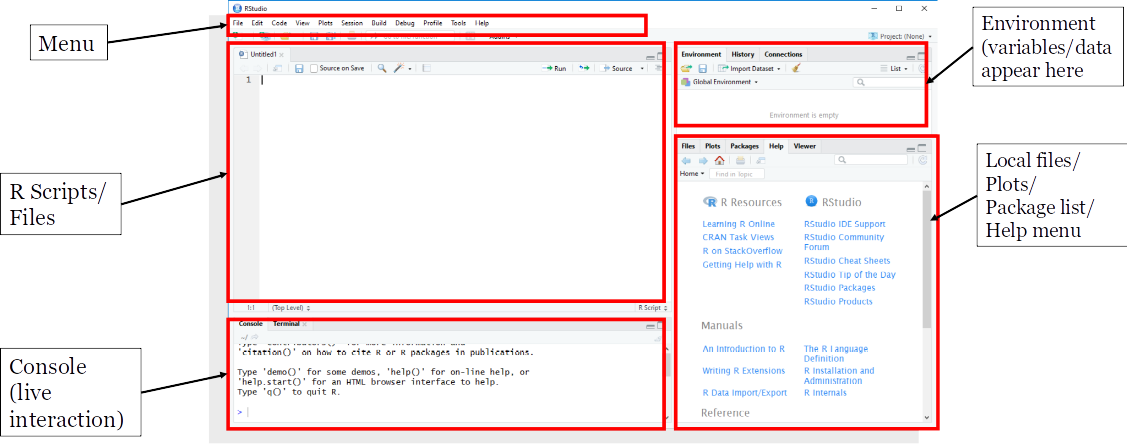
\includegraphics[width=1\textwidth,height=\textheight]{figures/Rstudio_interface.png}
\end{frame}

\begin{frame}{Working with notebooks}
\protect\hypertarget{working-with-notebooks}{}
\begin{itemize}
\tightlist
\item
  Notebooks are the best way to work with \textbf{R}
\item
  Allow you to work interactively

  \begin{itemize}
  \tightlist
  \item
    they save your work so you can see it later
  \item
    they also let you document your work
  \end{itemize}
\item
  R code is stored in chunks

  \begin{itemize}
  \tightlist
  \item
    each chunk can be run separately, or together
  \item
    click on the green arrow to execute each chunk
    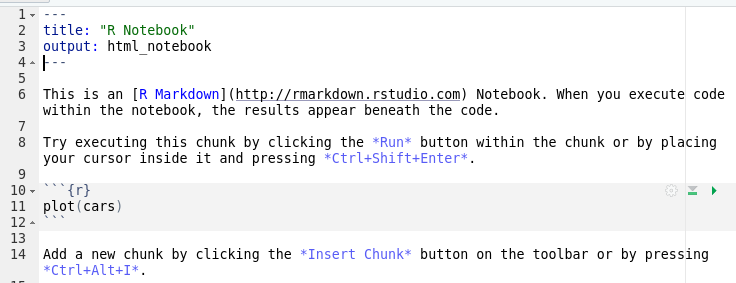
\includegraphics{figures/Notebook.png}
  \end{itemize}
\end{itemize}
\end{frame}

\begin{frame}{Loading and creating notebooks}
\protect\hypertarget{loading-and-creating-notebooks}{}
\begin{itemize}
\tightlist
\item
  To load a Notebook, double-click on the file or

  \begin{itemize}
  \tightlist
  \item
    select \textbf{File\textbar Open File}
  \end{itemize}
\item
  To create a new Notebook

  \begin{itemize}
  \tightlist
  \item
    select \textbf{File\textbar New File\textbar R Notebook}
  \item
    will create a skeleton Notebook containing text and chunks of
    \textbf{R} code
  \item
    remember to save the Notebook!
  \end{itemize}
\item
  When all the code is working, click on the Knit button to run the
  whole Notebook and create the output
\end{itemize}
\end{frame}

\begin{frame}[fragile]{Basic R tasks}
\protect\hypertarget{basic-r-tasks}{}
The file \texttt{Introduction\_to\_R\_Tutorial.Rmd} contains exercises
to work through.

\begin{itemize}
\tightlist
\item
  If you haven't used \textbf{R} very much, start at the beginning
\item
  If you are finding these too easy, skip to the \textbf{Advanced R}
  section
\end{itemize}
\end{frame}

\begin{frame}[fragile]{How to run the tutorials}
\protect\hypertarget{how-to-run-the-tutorials}{}
You can either

\begin{itemize}
\tightlist
\item
  execute each line one at a time by putting your cursor in the line and
  hitting {[}Ctrl{]}{[}Enter{]}
\item
  execute each chunk separately
\end{itemize}

When you are finished, you can \texttt{knit} the tutorial. You will get
a .pdf which will be a useful reference.
\end{frame}

\begin{frame}{Getting help}
\protect\hypertarget{getting-help}{}
\begin{itemize}
\tightlist
\item
  There is a lot of help in \textbf{RStudio}
\item
  For online help, use \url{https://rseek.org/}.
\item
  Check the R reference card in the /data directory
\end{itemize}
\end{frame}

\end{document}
